\begin{frame}{Resultados}
    % Please add the following required packages to your document preamble:
% \usepackage[table,xcdraw]{xcolor}
% If you use beamer only pass "xcolor=table" option, i.e. \documentclass[xcolor=table]{beamer}
\begin{table}[]
    \centering
    \caption[Tempo médio de operações]{Tempo (ns) médio de operações sobre o conjunto de dados Complete tree (ctree)}
    \begin{tabular}{lllll}
    \hline
    \multicolumn{1}{l}{\textbf{Operação}} & \multicolumn{1}{l}{\textbf{Binária}} & \multicolumn{1}{l}{\textbf{4-ária}} & \multicolumn{1}{c}{\textbf{8-ária}} & \multicolumn{1}{l}{\textbf{16-ária}} \\ \hline
    fwdSearch                               & 261,58                                & 325,06                               & 317,77                               & 318,34                                \\
    \rowcolor[HTML]{EFEFEF} 
    bwdSearch                               & 1679,19                                & 3200,95                              & 4032,87                              & 6027,23                               \\
    findClose                               & 334.38                                & 399,62                               & 396,91                               & 394,57                                \\
    \rowcolor[HTML]{EFEFEF} 
    findOpen                                & 381,89                                & 443,55                               & 443,54                               & 439,59                                \\
    enclose                                 & 325,01                                & 375,02                               & 377,77                               & 373,34                                \\
    \rowcolor[HTML]{EFEFEF} 
    isAncestor                              & 237,69                                & 264,61                               & 267,17                               & 266,70                                \\
    parent                                  & 327,19                                & 377,9                                & 378,63                               & 372,16                 \\ 
    \rowcolor[HTML]{EFEFEF} 
    subTreeSize                             & 352,38                                & 417,97                               & 418,75                               & 417,01                                \\
    %\rowcolor[HTML]{EFEFEF} 
    nextSibling                             & 264,41                                & 288,8,78                             & 287,45                               & 289,87                                \\ \hline            
    \end{tabular}
    \end{table}
\end{frame}


\begin{frame}{Resultados}
    % Please add the following required packages to your document preamble:
% \usepackage[table,xcdraw]{xcolor}
% If you use beamer only pass "xcolor=table" option, i.e. \documentclass[xcolor=table]{beamer}
\begin{table}[]
    \centering
    \caption[Tempo médio de operações]{Tempo (ns) médio de operações sobre o conjunto de dados Complete tree (ctree)}
    \begin{tabular}{lllll}
    \hline
    \multicolumn{1}{l}{\textbf{Operação}} & \multicolumn{1}{l}{\textbf{Binária}} & \multicolumn{1}{l}{\textbf{4-ária}} & \multicolumn{1}{c}{\textbf{8-ária}} & \multicolumn{1}{l}{\textbf{16-ária}} \\ \hline
    prevSibling                             & 240,24                                & 266,53                               & 268,30                               & 265,65                                \\
    \rowcolor[HTML]{EFEFEF} 
    lastChild                               & 395,22                                & 436,02                               & 437,15                               & 436,34                                \\
    levelNext                               & 366,81                                & 452,55                               & 450,61                               & 442,64                                \\
    \rowcolor[HTML]{EFEFEF} 
    levelAncestor                           & 882,93                                & 1656,51                              & 2089,76                              & 3113,49                               \\
    postRank                                & 177,92                                & 176,93                               & 174,66                               & 184,18                                \\
    \rowcolor[HTML]{EFEFEF} 
    postSelect                              & 844,9                                 & 911,84                               & 919,35                             & 372,16                 \\ \hline              
    \end{tabular}
    \end{table}
\end{frame}

\begin{frame}{Resultados}  
    \begin{figure}[h!]
        \centering
        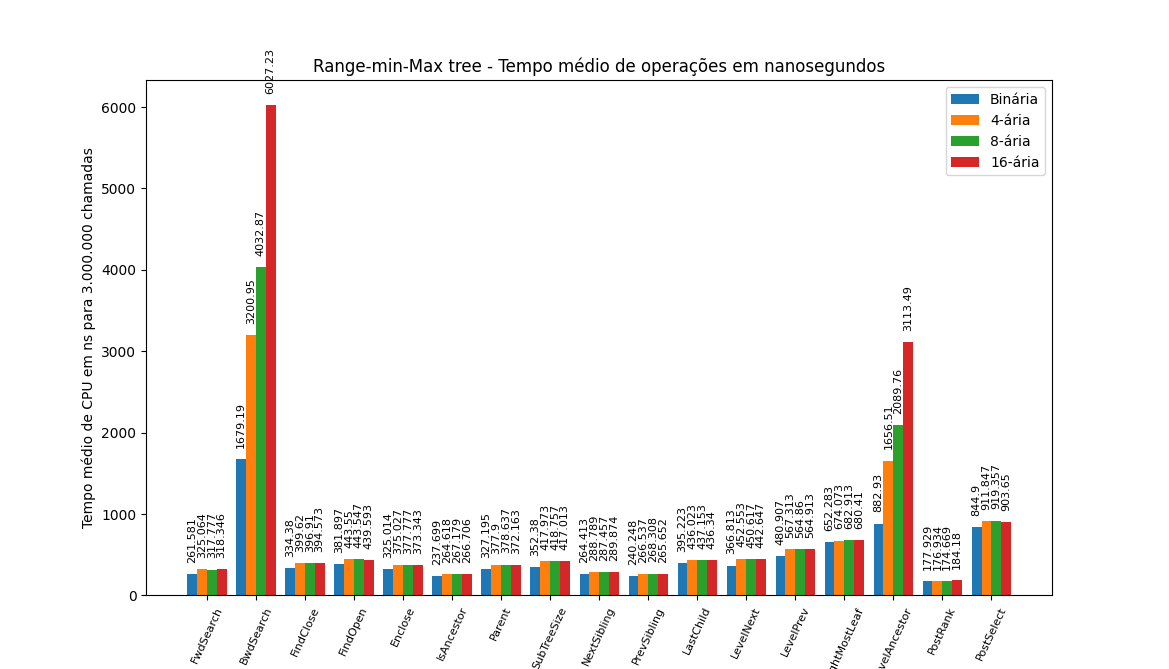
\includegraphics[scale=0.35]{images/ctree_i3000000.png}\\
        \caption{Tempo médio para $3.000.000$ requisições sobre o conjunto de dados Complete tree (ctree)}
    \end{figure} 
\end{frame}
